\documentclass{beamer}
\usepackage[utf8]{inputenc}
\usepackage{graphicx}
\usepackage{color}
%\usetheme{Hannover}
\newcommand{\hilight}[1]{\textbf{\textcolor{structure.fg!85}{#1}}}
\setbeamertemplate{footline}[frame number]

\usepackage{hyperref}
\hypersetup{
    colorlinks=true,
    linkcolor=blue,
    filecolor=magenta,      
    urlcolor=cyan,
}

\author[Sowmya Vajjala]{Sowmya Vajjala}

\title[SfSNLP]{NLP without Annotated Dataset}
\subtitle{NLP and Language Learning}


\date{29 January 2021}

\institute{Seminar f\"ur Sprachwissenschaft, University of T\"ubingen, Germany}
%%%%%%%%%%%%%%%%%%%%%%%%%%%

\begin{document}

\begin{frame}\titlepage
\end{frame}

\begin{frame}{NLP and Language Learning}
\framesubtitle{What are some applications?}
Broadly, four categories:
\begin{itemize}
    \item learning assessment
    \item learning support
    \item support tool for research (e.g., on language acquisition)
    \item learning analytics
\end{itemize}
\end{frame}

\begin{frame}{}
    \Large Learning Assessment
\end{frame}

\begin{frame}{Language Assessment}
    \begin{itemize}
        \item Automatic essay scoring systems (such as e-rater by ETS)
        \item Automatic speech scoring systems (SpeechRater by ETS)
        \item Automatic creation of test items: multiple choice questions, fill in the blanks etc 
        \item Active area of research for non-English languages too, in the past few years. 
    \end{itemize}
\end{frame}

\begin{frame}{Content Assessment}
    \begin{itemize}
        \item Evaluating short answers for correctness in relation to the question asked (i.e., going beyond looking for fluency, grammar/spelling correctness etc)
        \item To an extent, tougher than assessing language form. 
        \item It was an active area of research a few years ago, and SfS had a strong group. 
    \end{itemize}
\end{frame}

\begin{frame}{@SfS}
    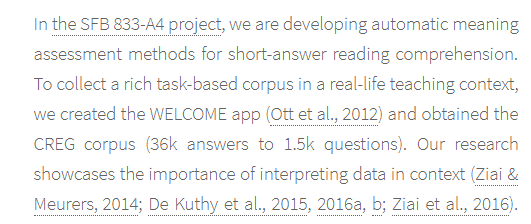
\includegraphics[width=\textwidth]{figures/sfs1.PNG}
    source: \url{http://www.sfs.uni-tuebingen.de/icall/}
\end{frame}

\begin{frame}{NLP and Language Learning}
\framesubtitle{What are some applications?}
Broadly, four categories:
\begin{itemize}
    \item language and content assessment
    \item \textbf{learning support}
    \item support tool for research on language acquisition
    \item learning analytics
\end{itemize}
\end{frame}

\begin{frame}{Learning support}
    \begin{itemize}
    \item Reading support: TextEvaluator (ETS) like tools to choose texts appropriate for a reading level
        \item Writing support:Spelling/grammar check tools (e.g., grammarly); specialized writing support (e.g., WritingMentor from ETS for academic writing support)
        \item Language learning apps (e.g., duolingo)
    \end{itemize}
\end{frame}

\begin{frame}{@SfS}
    \begin{itemize}
        \item "Portuguese Intelligent Tutoring System (ITS) TAGARELA (Amaral & Meurers 2011) designed to complement university instruction"
        \item "in collaboration with a German school book publisher we created the FeedBook, an interactive workbook for English 7th grade in a DFG-funded transfer project."
        \item "In the new BMBF project AISLA, we develop an intelligent dialog system supporting the acquisition of English in authentic, spoken language contexts. "
            \item "developing Prosodiya, a mobile serious game for German dyslexic primary-school children currently"
    \end{itemize}
    source: \url{http://www.sfs.uni-tuebingen.de/icall/}
\end{frame}

\begin{frame}{@SfS-2}

\includegraphics[width=\textwidth]{figures/sfs2.PNG}
source: \url{http://www.sfs.uni-tuebingen.de/icall/}
\end{frame}

\begin{frame}{NLP and Language Learning}
\framesubtitle{What are some applications?}
Broadly, four categories:
\begin{itemize}
    \item learning assessment
    \item learning support 
    \item \textbf{support tool for research}
    \item learning analytics
\end{itemize}
\end{frame}

\begin{frame}{Language Acquisition Research}
    \begin{itemize}
        \item Using NLP tools to study specific linguistic phenomenon in large learner corpora, to understand language acquisition
        \item Dependency parsing of learner language
        \item A recent paper: \href{https://www.jbe-platform.com/content/journals/10.1075/ijcl.18097.hua}{"Subcategorization frame identification for learner English"}
    \end{itemize}
    etc. 
\end{frame}

\begin{frame}{@SfS}
Studying learner language: 
    \begin{itemize}
        \item "With Katrin Wisniewski we explored linguistic correlates of the CEFR as part of the MERLIN project."
        \item "We characterize language development both for specific constructions, e.g., relative clauses (Alexopoulou, Geertzen, Korhonen \& Meurers, 2015) and in terms of linguistic complexity, emphasizing the need to account for task effects (Alexopoulou, Michel, Murakami \& Meurers, 2017)."
        \item "We also analyze L1 transfer effects using machine learning for Native Language Identification"
    \end{itemize}
    source: \url{http://www.sfs.uni-tuebingen.de/icall/}
\end{frame}

\begin{frame}{NLP and Language Learning}
\framesubtitle{What are some applications?}
Broadly, four categories:
\begin{itemize}
    \item language and content assessment
    \item learning support for reading, writing, speaking, and listening
    \item support tool for research on language acquisition, learner corpora etc. 
    \item \textbf{student data analytics}
\end{itemize}
\end{frame}

\begin{frame}{Student data analytics}
    \begin{itemize}
        \item modeling student engagement through their activity (incl. postings etc)
        \item summarizing course feedback given by students
        \item visualization of learning program etc. 
        \item recent work from SfS: \href{http://ceur-ws.org/Vol-2592/paper1.pdf}{"Enhancing a Web-based Language Tutoring System with
Learning Analytics"}
    \end{itemize}
\end{frame}

\begin{frame}{Summary}
    \begin{itemize}
        \item NLP is used in a wide range of topics related to human language learning.
        \item From research to industry, there are many interesting problems to study and solve.
        \item At SfS, there is a strong group focusing on this kind of research - so talk to them!
    \end{itemize}
\end{frame}

\begin{frame}{Where to look to know more}
\begin{itemize}
    \item \href{https://www.aclweb.org/anthology/venues/bea/}{BEA workshop series}
    \item \href{https://www.aclweb.org/anthology/venues/nlp4call/}{NLP4CALL workshop series}
    \item Talk to \href{http://www.sfs.uni-tuebingen.de/icall/}{Prof. Meurers and team.} 
    \item Two summary articles (by prof and ex-advisee):
    \begin{itemize}
        \item Detmar Meurers (2013, 2020). Natural Language Processing and Language Learning. The Encyclopedia of Applied Linguistics, edited by Carol A. Chapelle. Wiley. 
        \item Sowmya Vajjala (2018). Machine Learning in Applied Linguistics. The Encyclopedia of Applied Linguistics (ed: Carol Chapelle). Wiley. (\footnotesize{Okay, I am not sharing out of vanity. It really gives an overview)} 
    \end{itemize}
\end{itemize}    
\end{frame}

\end{document}